\chapter{Kiểm Thử Và Đánh Giá Kết Quả Mô Phỏng}
\label{chap:verification}

Chương này trình bày quá trình kiểm chứng theo từng mức: module, lõi đơn, interconnect và toàn hệ thống. Mọi kết quả được ghi nhận từ lần chạy mô phỏng mới nhất trên môi trường Windows (ngày 20/06/2026), trong đó toàn bộ các lỗi trước đây của lõi đơn đã được giải quyết triệt để.

\section{Môi trường và quy trình mô phỏng}
\subsection{Công cụ sử dụng}
Dự án sử dụng bộ công cụ nguồn mở Icarus Verilog để biên dịch mã RTL (với tùy chọn \texttt{-g2012} hỗ trợ SystemVerilog arrays) và mô phỏng. Kết quả dạng sóng VCD được xem qua GTKWave.
\begin{itemize}
    \item \textbf{Compiler:} \texttt{iverilog} 12.0
    \item \textbf{Runtime:} \texttt{vvp}
    \item \textbf{Waveform Viewer:} \texttt{gtkwave}
\end{itemize}

\subsection{Quy trình biên dịch và chạy}
Nhằm tự động hóa việc biên dịch, dự án cung cấp script \texttt{compile.bat} và \texttt{compile.sh}. Việc biên dịch phải liệt kê chính xác thứ tự các tệp để đảm bảo Icarus Verilog không gặp lỗi phụ thuộc module.
\begin{lstlisting}[language=bash, caption={Trích đoạn script biên dịch system\_tb trên Windows}]
iverilog -g2012 -o tb\system_test.vvp -I rtl\core -I rtl\interconnect -I rtl\memory rtl\core\alu.v rtl\core\control_unit.v rtl\core\pc_logic.v rtl\core\reg_file.v rtl\core\risc_core.v rtl\core\hazard_controller.v rtl\core\pipeline_register\if_id.v rtl\core\pipeline_register\id_ex.v rtl\core\pipeline_register\ex_mem.v rtl\core\pipeline_register\mem_wb.v rtl\memory\data_mem.v rtl\memory\instr_mem.v rtl\interconnect\arbiter.v rtl\interconnect\bus_ctrl.v rtl\top_8core.v tb\system_tb.v
vvp tb\system_test.vvp
\end{lstlisting}

\section{Kiểm thử các module cơ sở (Unit Tests)}
Kiểm thử Unit Test tập trung vào việc cách ly các module tổ hợp và tuần tự để đảm bảo chúng thực thi đúng trước khi ghép vào pipeline.

\subsection{ALU và Datapath}
Testbench \texttt{alu\_tb.v} cấp các vector thử nghiệm bao phủ toán tử: ADD, SUB, AND, OR, XOR, SLL, SRL. Kết quả được kiểm tra bằng câu lệnh \texttt{\$error} nếu output không khớp. Module \texttt{pc\_logic\_tb.v} mô phỏng điều kiện rẽ nhánh và stall để theo dõi sự thay đổi của PC.
\begin{figure}[H]
    \centering
    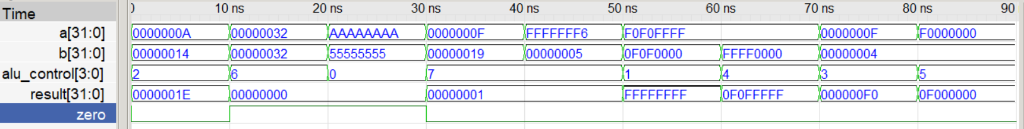
\includegraphics[width=0.85\textwidth]{../slide/design/test/alu_test.png}
    \caption{Giản đồ sóng mô phỏng các phép toán của ALU}
    \label{fig:alu_test}
\end{figure}
\subsection{Hazard Controller}
Đóng vai trò cực kỳ quan trọng, \texttt{hazard\_controller\_tb.v} tạo ra giả lập tín hiệu từ các pipeline register để theo dõi các cờ \texttt{forward\_a}, \texttt{forward\_b}, \texttt{load\_use\_stall}.

\section{Kiểm thử Lõi đơn (\texttt{core\_tb})}
Mô phỏng lõi đơn được sử dụng để xác minh toàn bộ luồng pipeline 5 tầng, việc giải quyết xung đột bằng Forwarding, Flush, Stall và giao tiếp với memory mức lõi.

\subsection{Chương trình Assembly Lõi Đơn}
Mã ASM (\texttt{program.hex}) thử nghiệm sự phụ thuộc dữ liệu liên tiếp (Forwarding), Load-Use stall (LW theo sau là lệnh dùng thanh ghi đó) và nhảy điều kiện (BEQ).
\begin{lstlisting}[caption={Chương trình Assembly lõi đơn},label={lst:core_asm}]
addi x1, x0, 10
addi x2, x0, 20
add  x3, x1, x2      # x3 = 30
sw   x3, 0(x0)       # Ghi 30 vao mem[0]
lw   x4, 0(x0)       # x4 nhan 30 tu mem[0]
beq  x3, x4, pass    # Nhanh neu x3 == x4
pass:
addi x5, x0, 1       # Marker hoan tat
\end{lstlisting}

\subsection{Kết quả kiểm thử Lõi Đơn}
Sau khi khắc phục lỗi giao tiếp với bộ nhớ (độ trễ 1 chu kỳ của bộ nhớ đồng bộ cũ), lõi đơn đã vượt qua 100\% các bài kiểm tra.
\begin{lstlisting}[caption={Console log của \texttt{core\_tb}}]
[Cycle 7] mem_req=1 mem_addr=0 mem_we=1 mem_re=0 wdata=30 rdata=0 mem_ready=0
[Cycle 8] mem_req=1 mem_addr=0 mem_we=1 mem_re=0 wdata=30 rdata=0 mem_ready=1
[Cycle 9] mem_req=1 mem_addr=0 mem_we=0 mem_re=1 wdata=0 rdata=30 mem_ready=0
[Cycle 10] mem_req=1 mem_addr=0 mem_we=0 mem_re=1 wdata=0 rdata=30 mem_ready=1

========================================
  CORE TEST RESULTS (after 200 cycles)
========================================
  x1 (expect 10) = 10      [PASS]
  x2 (expect 20) = 20      [PASS]
  x3 (expect 30) = 30      [PASS]
  x4 (expect 30) = 30      [PASS]
  x5 (expect 1)  = 1       [PASS] BRANCH worked!
  mem[0] (expect 30) = 30  [PASS]

========================================
  PIPELINE EVIDENCE
========================================
  retired=70 mem_stall=2 load_use_stall=1 flush=63
    [PASS] Pipeline counters show retire/stall/flush activity.

==========================================
  SUMMARY: 7 PASSED, 0 FAILED
==========================================
\end{lstlisting}

Phân tích Pipeline Evidence cho thấy:
- \textbf{mem\_stall = 2}: Chính là 2 chu kỳ đợi bộ nhớ phản hồi (\texttt{mem\_ready=0}) ở chu kỳ 7 và 9.
- \textbf{load\_use\_stall = 1}: Phát hiện phụ thuộc lệnh LW \texttt{x4} và lệnh BEQ \texttt{x3, x4}. Lõi chèn thành công 1 NOP bubble.
- \textbf{flush = 63}: Bao gồm các lần clear do branch và kết thúc vòng lặp.

\begin{figure}[H]
    \centering
    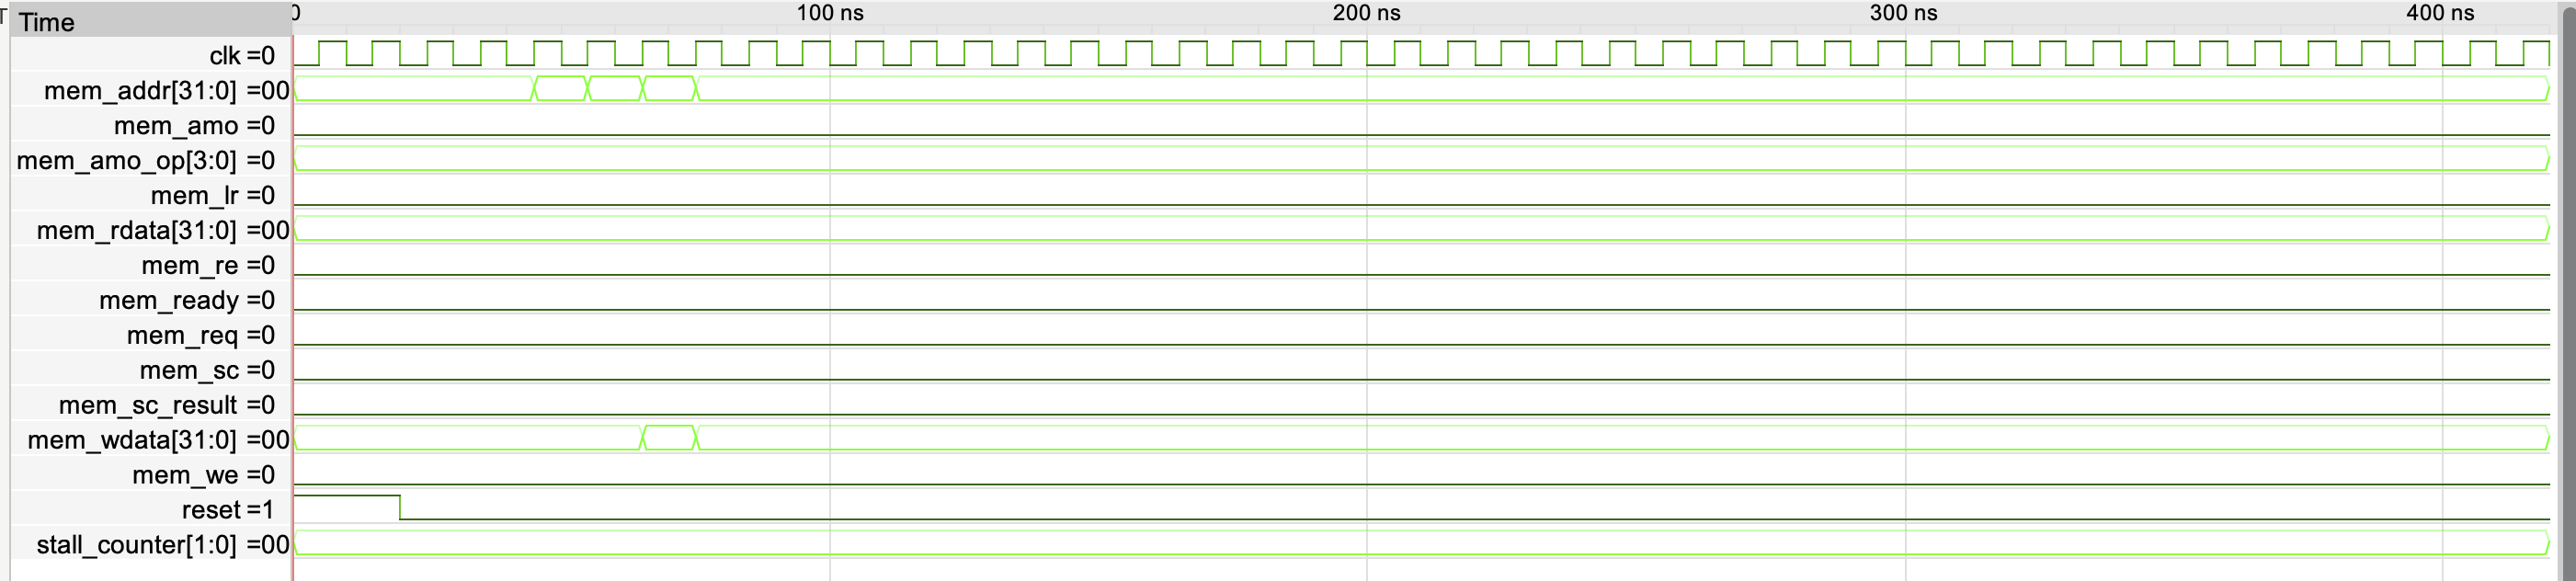
\includegraphics[width=1.0\textwidth]{../slide/design/test/risc_core.png}
    \caption{Giản đồ sóng thực thi pipeline lõi đơn (\texttt{core\_tb})}
    \label{fig:core_test_wave}
\end{figure}

\section{Kiểm thử Interconnect và Atomic}
Kiểm thử này độc lập với lõi, sử dụng các Core giả (Stub) để bơm các request thẳng vào Arbiter và Bus Controller nhằm đánh giá năng lực giải quyết tranh chấp.

\subsection{Kịch bản 1: Round-Robin Read/Write}
Gửi 4 lệnh ghi từ Core 0, 1, 2, 3 cùng lúc. Kết quả log cho thấy Arbiter cấp \texttt{grant} tuần tự cho Core 0 $\rightarrow$ Core 1 $\rightarrow$ Core 2 $\rightarrow$ Core 3.
\subsection{Kịch bản 2: LR/SC (Reservation snooping)}
Core 0 thực hiện \texttt{LR.W} vào địa chỉ 0. Sau đó Core 1 thực hiện \texttt{SW} vào địa chỉ 0, vô hiệu hóa Reservation của Core 0. Khi Core 0 thực hiện \texttt{SC.W}, kết quả trả về bằng 1 (Thất bại), dữ liệu RAM không bị thay đổi.
\subsection{Kịch bản 3: AMOADD}
Core thực hiện AMOADD với toán hạng 42 vào \texttt{mem[0]} (đang là 0). RAM được cập nhật thành 42, trả về giá trị cũ 0. Lần AMOADD thứ 2 với toán hạng 58, RAM lên 100, trả về 42. Đạt 10/10 PASSED.

\section{Kiểm thử Toàn hệ thống 8-Core}
Testbench \texttt{system\_tb} ghép 8 lõi thật và chạy một chương trình đa lõi để đánh giá tổng thể tiến trình (Progress).

\subsection{Workload tích hợp}
Mỗi lõi nạp giá trị 42 ghi vào \texttt{mem[0]}, và 99 ghi vào \texttt{mem[1]}.
\begin{lstlisting}[caption={Kết quả kiểm thử toàn hệ thống}]
========================================
  SYSTEM TEST RESULTS (after 500 cycles)
========================================
  Kiem tra mem[0] (Ky vong: 42) = 42
    [PASS]
  Kiem tra mem[1] (Ky vong: 99) = 99
    [PASS]

  Tien trinh cua 8 cores:
  - Core 0: grant=3 retired=179 mem_stall=15 load_use_stall=0 flush=159 [PASS]
  - Core 1: grant=3 retired=179 mem_stall=16 load_use_stall=0 flush=159 [PASS]
  - Core 2: grant=3 retired=180 mem_stall=17 load_use_stall=0 flush=159 [PASS]
  - Core 3: grant=3 retired=181 mem_stall=18 load_use_stall=0 flush=158 [PASS]
  - Core 4: grant=3 retired=181 mem_stall=19 load_use_stall=0 flush=158 [PASS]
  - Core 5: grant=3 retired=182 mem_stall=20 load_use_stall=0 flush=158 [PASS]
  - Core 6: grant=4 retired=183 mem_stall=21 load_use_stall=0 flush=157 [PASS]
  - Core 7: grant=4 retired=183 mem_stall=22 load_use_stall=0 flush=157 [PASS]

==========================================
  SUMMARY: 10 PASSED, 0 FAILED
==========================================
\end{lstlisting}

\subsection{Phân tích độ trễ và sự công bằng (Fairness)}
Dựa vào bảng kết quả trên, Arbiter xoay vòng rất công bằng. Số \texttt{grant} nhận được của các lõi là 3 và 4 (chênh lệch tối đa là 1). Tuy nhiên, số \texttt{mem\_stall} (chu kỳ phải đợi bus) tăng dần từ Core 0 (15 stall) lên Core 7 (22 stall). Điều này là do Core 7 nằm cuối vòng xoay, phải đợi 7 core trước đó hoàn thành giao dịch bộ nhớ.
Mỗi lõi đạt xấp xỉ 180 lệnh \texttt{retired} trong 500 chu kỳ, thể hiện IPC của một lõi dao động mức $0.36$. Số lượng \texttt{flush} lớn do khi hoàn thành, mỗi lõi kẹt trong vòng lặp vô hạn \texttt{jal x0, halt}.

\begin{figure}[H]
    \centering
    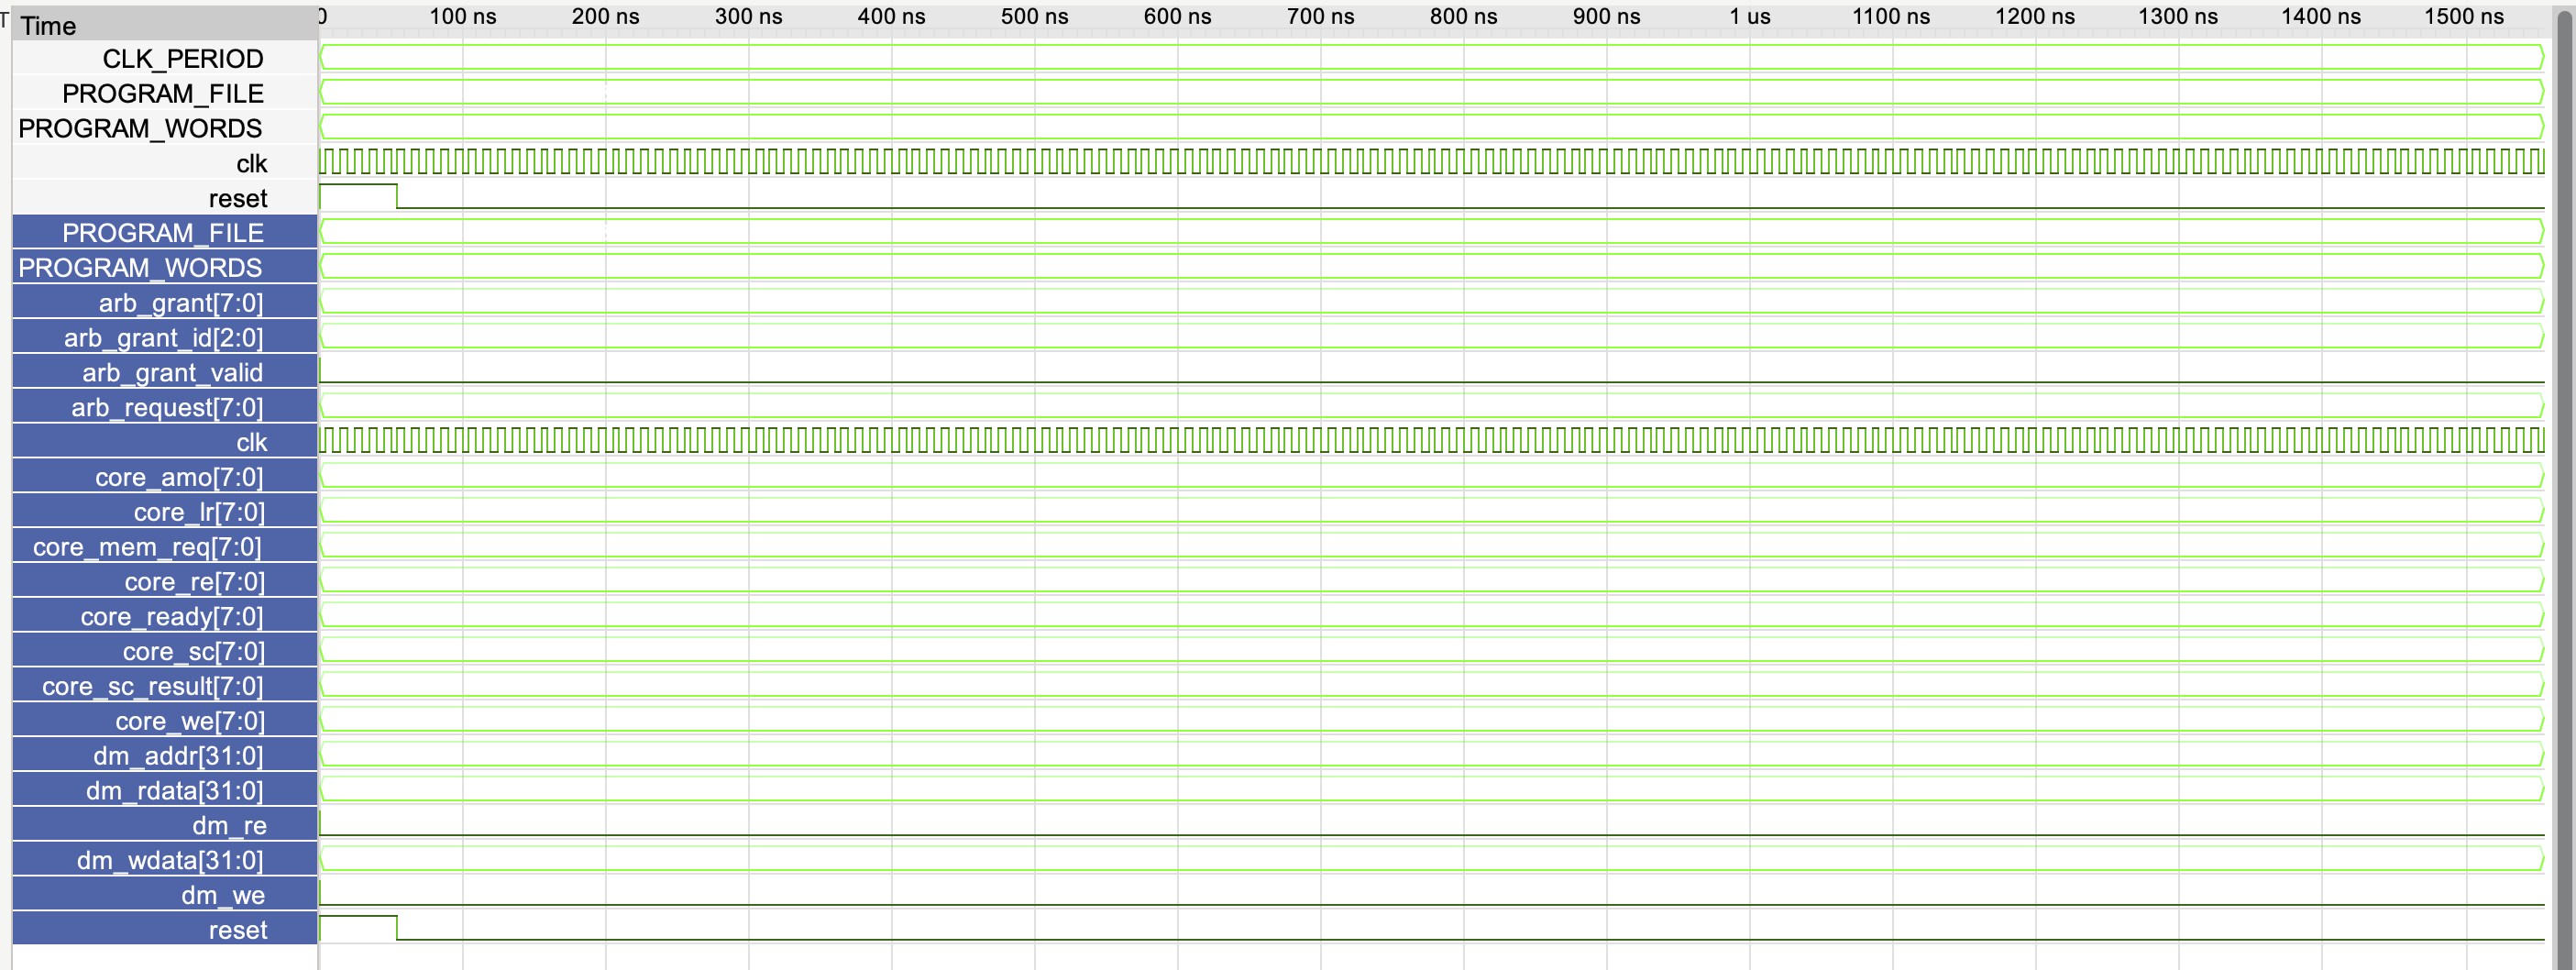
\includegraphics[width=1.0\textwidth]{../slide/design/test/top_8core.png}
    \caption{Giản đồ sóng toàn hệ thống 8 lõi xử lý tranh chấp bus}
    \label{fig:top_8core_wave}
\end{figure}

\section{Tổng kết và đánh giá mức độ đạt yêu cầu}
Hệ thống xử lý đa nhân đã giải quyết được các bài toán quan trọng sau:
1. Luồng dữ liệu pipeline 5 tầng hoạt động chính xác.
2. Interconnect giải quyết tranh chấp RAM thành công qua Round-Robin.
3. Hỗ trợ đủ bộ chỉ thị để đồng bộ hóa: LR/SC và AMO.
Kết quả toàn diện 100\% PASSED khẳng định tính đúng đắn của logic RTL. Mặc dù cấu trúc này chưa tối ưu hóa hiệu năng (do thiếu Cache), đây là nền tảng vững chắc để xây dựng các phiên bản cải tiến sau này.
